\documentclass[12pt,a4paper]{report}

% ---------- Packages ----------
\usepackage[margin=1in,headheight=14pt]{geometry}
\usepackage{amsmath}
\usepackage{seqsplit}
\usepackage{times}
\usepackage{graphicx}
\usepackage{tikz}
\usetikzlibrary{arrows.meta, positioning, shapes.geometric, fit, backgrounds}
\usepackage{algorithm}
\usepackage{algpseudocode}
\usepackage{booktabs}
\usepackage{longtable}
\usepackage{hyperref}
\usepackage{xcolor}
\usepackage{setspace}
\usepackage{titlesec}
\usepackage{fancyhdr}
\usepackage{enumitem}
\usepackage{caption}

\hypersetup{
    colorlinks=true,
    linkcolor=black,
    citecolor=black,
    urlcolor=blue,
    pdftitle={Distributed File System},
    pdfauthor={Satyam Kumar Chauhan, Devansh Singhal}
}

\onehalfspacing
\setlength{\parskip}{6pt}
\setlength{\parindent}{0pt}

\titleformat{\chapter}[hang]{\normalfont\huge\bfseries}{\thechapter.}{20pt}{\huge}
\titlespacing*{\chapter}{0pt}{-20pt}{20pt}

\pagestyle{fancy}
\fancyhf{}
\fancyhead[L]{\small Distributed File System}
\fancyhead[R]{\small NIT Kurukshetra}
\fancyfoot[C]{\thepage}
\renewcommand{\headrulewidth}{0.4pt}

% ---------- Document ----------
\begin{document}

% =====================================================
% TITLE PAGE
% =====================================================
\begin{titlepage}
    \centering
    \vspace*{0.5cm}
    {\large \textbf{National Institute of Technology Kurukshetra}\par}
    {\large Department of Computer Engineering\par}
    \vspace{0.3cm}
    {\normalsize B.Tech. (Artificial Intelligence and Machine Learning), 6\textsuperscript{th} Semester\par}
    {\normalsize Academic Year 2025--26\par}

    \vspace{1.5cm}
    {\Huge \textbf{Distributed File System}\par}
    \vspace{0.4cm}
    {\Large A Fault-Tolerant Distributed File System with\par}
    {\Large Raft-based Metadata Management and P2P Chunk Replication\par}

    \vspace{1cm}
    {\large B.Tech. Project Report (AIPC 304)\par}
    {\large Project Group No.: \textbf{AI2}\par}

    \vspace{1.5cm}
    {\large \textbf{Submitted by}\par}
    \vspace{0.3cm}
    \begin{tabular}{ll}
        Satyam Kumar Chauhan & 123108031 \\[4pt]
        Devansh Singhal & 123108032 \\
    \end{tabular}

    \vspace{2cm}
    {\large \textbf{Under the Supervision of}\par}
    \vspace{0.2cm}
    {\large Prof. R. K. Aggarwal\par}
    {\normalsize Department of Computer Engineering\par}

\end{titlepage}

% =====================================================
% CERTIFICATE
% =====================================================
\chapter*{Certificate}
\addcontentsline{toc}{chapter}{Certificate}

This is to certify that the project report entitled \textbf{``Distributed File System: A Fault-Tolerant Distributed File System with Raft-based Metadata Management and P2P Chunk Replication''}, submitted by \textbf{Satyam Kumar Chauhan (123108031)} and \textbf{Devansh Singhal (123108032)}, Project Group \textbf{AI2}, in partial fulfillment of the requirements for the End-Semester Evaluation of B.Tech. Project (AIPC 304), Department of Computer Engineering, National Institute of Technology Kurukshetra, is a record of bona fide work carried out by them under my supervision.

\vspace{2cm}

\begin{flushright}
\begin{tabular}{c}
    \hline
    \textbf{Prof. R. K. Aggarwal} \\
    Project Supervisor \\
    Department of Computer Engineering \\
    NIT Kurukshetra
\end{tabular}
\end{flushright}

\vspace{1cm}
Date: \underline{\hspace{4cm}}

% =====================================================
% DECLARATION
% =====================================================
\chapter*{Declaration}
\addcontentsline{toc}{chapter}{Declaration}

We hereby declare that the work presented in this project report titled \textbf{``Distributed File System''} is an authentic record of our own work carried out under the supervision of \textbf{Prof. R. K. Aggarwal}. This work has not been submitted elsewhere, in part or in full, for the award of any other degree or diploma. All sources of information used have been duly acknowledged in the References section.

\vspace{2cm}

\begin{tabular}{ll}
    Satyam Kumar Chauhan (123108031) & \underline{\hspace{4cm}} \\[6pt]
    Devansh Singhal (123108032) & \underline{\hspace{4cm}} \\
\end{tabular}

\vspace{1cm}
Date: \underline{\hspace{4cm}}

% =====================================================
% ABSTRACT
% =====================================================
\chapter*{Abstract}
\addcontentsline{toc}{chapter}{Abstract}

Modern data-intensive applications need storage systems that stay available and durable even though individual machines fail routinely. This project presents the design and implementation of a fault-tolerant distributed file system (DFS) in Go, built along the same lines as the Google File System (GFS) and the Hadoop Distributed File System (HDFS). The central design decision is to keep the \emph{control plane} and the \emph{data plane} strictly separate. A small, strongly consistent metadata cluster, replicated using the Raft consensus algorithm, tracks file-to-chunk and chunk-to-node mappings, node liveness, and replication state. A set of independent storage nodes hold the actual file data and replicate it directly to one another over a peer-to-peer channel. Files are split into fixed-size 4~MB chunks with deterministically derived identifiers, uploaded in parallel to primary nodes that fan out replicas, and committed to the metadata log only once a replication quorum is reached. A heartbeat-driven failure detector (Alive~$\rightarrow$~Suspect~$\rightarrow$~Dead) triggers automatic re-replication of chunks lost to a node failure, and this is piggybacked on the regular heartbeat channel so it doesn't add extra coordination overhead. All inter-service communication uses gRPC with Protocol Buffers, using unary, client-streaming, server-streaming, and bidirectional-streaming RPCs wherever each fits best. The system is validated through an extensive integration test suite covering node registration and heartbeating, full upload/download round trips, chunk-size boundary conditions, checksum integrity, replication convergence, repair after simulated node death, and Raft leader-failover recovery. The result is a working, testable demonstration of the core mechanisms that underpin production distributed storage systems: consensus, replication, failure detection, and self-healing, along with an honest account of the simplifications (write-once semantics, no rack awareness, no transport security) made to keep the system tractable within the scope of a B.Tech. project.

\vspace{0.5cm}
\textbf{Keywords:} Distributed Systems, Raft Consensus, Distributed File System, Fault Tolerance, gRPC, Replication, Go.

% =====================================================
% TOC
% =====================================================
\tableofcontents
\listoffigures
\listoftables

% =====================================================
\chapter{Introduction}
% =====================================================

A distributed file system (DFS) allows files to be stored, replicated, and accessed across a cluster of independent machines while still presenting a single logical namespace to clients. Unlike a local file system, a DFS has to explicitly account for the fact that any individual machine, whether it stores metadata or raw file bytes, can fail at any time, and that the network connecting these machines is neither instantaneous nor perfectly reliable. Large-scale systems such as the Google File System (GFS) and its open-source descendant, the Hadoop Distributed File System (HDFS), established what is now the standard pattern: separate a small, centralized \emph{metadata service} from a large, horizontally scalable set of \emph{storage (chunk) servers}.

This project implements a scaled-down but architecturally faithful version of this pattern. It is composed of three cooperating components:

\begin{itemize}[nosep]
    \item A \textbf{metadata cluster} of Raft-replicated nodes that owns all bookkeeping: which files exist, which chunks compose them, which nodes hold each chunk, and which nodes are currently alive.
    \item A set of \textbf{storage nodes} that persist chunk data to local disk, replicate chunks to one another directly (peer-to-peer), and periodically report their health to the metadata cluster.
    \item A \textbf{client} (implemented as both a library and a CLI) that splits files into chunks, coordinates placement with the metadata cluster, and transfers chunk data in parallel to and from storage nodes.
\end{itemize}

The system is written entirely in Go, using \texttt{hashicorp/raft} for consensus, BoltDB for local persistence, and gRPC/Protocol Buffers for all inter-node communication. The remainder of this report describes the motivation for the project, surveys the background systems and algorithms it draws on, details the proposed design and its core algorithms, describes the experimental validation performed, and concludes with an honest assessment of the system's limitations and directions for future work.

% =====================================================
\chapter{Motivation}
% =====================================================

Distributed consensus and replication are among the most conceptually demanding topics in systems engineering, and they are also among the hardest to learn by just reading about them. Papers such as the Raft paper or the GFS paper describe the algorithms precisely, but the subtle failure interactions (what exactly happens when a leader crashes mid-write, or when a heartbeat is delayed just past a timeout) only really become clear once you build such a system yourself and deliberately break it.

The motivation for this project was therefore threefold:

\begin{enumerate}[nosep]
    \item \textbf{Pedagogical:} to move from reading about Raft, quorum replication, and failure detectors to implementing and testing them directly, including deliberately killing nodes mid-operation and observing the recovery path.
    \item \textbf{Practical:} to understand, first-hand, the engineering decisions that production systems like GFS/HDFS/Ceph make (fixed vs. variable chunk sizing, where checksums should live, how repair work gets scheduled without overloading the cluster) by making, and living with, the same decisions at a smaller scale.
    \item \textbf{Architectural:} to practice designing a multi-service system with well-defined RPC boundaries (metadata service, storage service, replication service) rather than a monolith, which mirrors how real distributed storage systems are decomposed.
    \end{enumerate}

Building a DFS specifically (rather than, say, a simple key-value store) was chosen because it exercises nearly every core distributed-systems concept in one project: consensus (Raft), replication and quorum, data placement, failure detection, self-healing, streaming data transfer, and data integrity verification.

% =====================================================
\chapter{Related and Background Work}
% =====================================================

\section{Google File System (GFS)}
GFS established the chunk-server architecture this project follows: files are divided into large, fixed-size chunks (64~MB in GFS), a single master maintains all metadata in memory, and clients contact chunk servers directly for data transfer after obtaining locations from the master. GFS keeps its master simple and fast precisely by keeping bulk data traffic off of it. This project follows the same separation, though with three important differences: metadata is Raft-replicated across multiple nodes rather than served by a single master with shadow masters, chunk size is much smaller (4~MB, configurable), and there is no lease-based primary/mutation-order protocol since the system is write-once.

\section{Hadoop Distributed File System (HDFS)}
HDFS is the open-source, production-hardened realization of the GFS design, with a NameNode holding metadata and DataNodes holding replicated blocks. HDFS's heartbeats and block-reports are the direct inspiration for this project's heartbeat and repair-scheduling design. One thing worth noting is that HDFS's NameNode was historically a single point of failure, and this was only fixed later with HA extensions; this project sidesteps that weakness from the start by using Raft for the metadata cluster instead of a single node.

\section{Raft Consensus Algorithm}
Raft was designed as a more understandable alternative to Paxos by decomposing consensus into three largely independent sub-problems: leader election, log replication, and safety. A cluster of $n$ nodes tolerates $\lfloor (n-1)/2 \rfloor$ failures while continuing to make progress, since all decisions require agreement from a majority. This project uses the mature, widely deployed \texttt{hashicorp/raft} library (also used by Consul and Nomad) rather than implementing Raft from scratch, allowing the project's own contribution to focus on how a DFS is built \emph{on top of} a consensus primitive.

\section{gRPC and Protocol Buffers}
gRPC provides strongly typed, code-generated RPC contracts over HTTP/2, along with native support for streaming RPCs (client-streaming, server-streaming, and bidirectional). This project relies on all three streaming modes: chunk upload uses client-streaming, chunk download uses server-streaming, and peer-to-peer chunk replication between storage nodes uses bidirectional streaming for flow control.

\section{BitTorrent-style Peer-to-Peer Replication}
The peer-to-peer chunk replication in this project is loosely inspired by BitTorrent's model of peers exchanging data directly rather than through a central server. The key difference is that this system's storage nodes are not anonymous, ephemeral peers but managed, identified nodes with a guaranteed replication factor enforced by the metadata cluster, rather than best-effort availability driven by a tracker.

% =====================================================
\chapter{Proposed Work and System Design}
% =====================================================

\section{System Architecture}

The system separates the control plane (metadata cluster) from the data plane (storage nodes), as shown in Figure~\ref{fig:architecture}.

\begin{figure}[h]
\centering
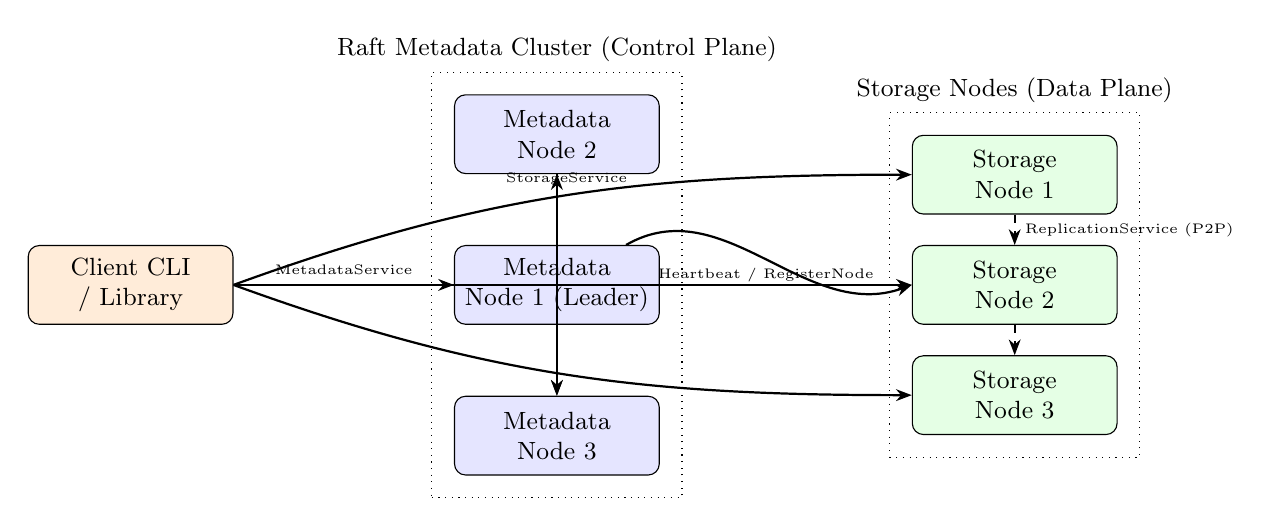
\begin{tikzpicture}[
    node distance=1.1cm and 1.6cm,
    box/.style={draw, rounded corners, minimum width=2.6cm, minimum height=1cm, align=center, font=\small},
    metabox/.style={box, fill=blue!10},
    storagebox/.style={box, fill=green!10},
    clientbox/.style={box, fill=orange!15},
    arrow/.style={-{Stealth[length=2mm]}, thick}
]
    \node[clientbox] (client) {Client CLI\\ / Library};

    \node[metabox, right=of client, xshift=1.2cm] (m1) {Metadata\\ Node 1 (Leader)};
    \node[metabox, above=of m1, yshift=-0.2cm] (m2) {Metadata\\ Node 2};
    \node[metabox, below=of m1, yshift=0.2cm] (m3) {Metadata\\ Node 3};

    \node[storagebox, right=of m1, xshift=1.6cm, yshift=1.4cm] (s1) {Storage\\ Node 1};
    \node[storagebox, right=of m1, xshift=1.6cm] (s2) {Storage\\ Node 2};
    \node[storagebox, right=of m1, xshift=1.6cm, yshift=-1.4cm] (s3) {Storage\\ Node 3};

    \draw[arrow] (client) -- node[above, font=\tiny]{MetadataService} (m1);
    \draw[arrow] (m1) -- (m2);
    \draw[arrow] (m1) -- (m3);
    \draw[arrow] (m2) -- (m3);

    \draw[arrow] (client.east) to[out=20,in=180] node[above, font=\tiny]{StorageService} (s1.west);
    \draw[arrow] (client.east) to[out=0,in=180] (s2.west);
    \draw[arrow] (client.east) to[out=-20,in=180] (s3.west);

    \draw[arrow] (m1) to[out=30,in=200] node[below, font=\tiny]{Heartbeat / RegisterNode} (s2.west);

    \draw[arrow, dashed] (s1) -- node[right, font=\tiny]{ReplicationService (P2P)} (s2);
    \draw[arrow, dashed] (s2) -- (s3);

    \begin{scope}[on background layer]
        \node[draw, dotted, fit=(m1)(m2)(m3), inner sep=8pt, label=above:{\small Raft Metadata Cluster (Control Plane)}] {};
        \node[draw, dotted, fit=(s1)(s2)(s3), inner sep=8pt, label=above:{\small Storage Nodes (Data Plane)}] {};
    \end{scope}
\end{tikzpicture}
\caption{High-level system architecture: control plane (Raft metadata cluster) is strictly separated from the data plane (storage nodes), which replicate chunks directly among themselves.}
\label{fig:architecture}
\end{figure}

\subsection{Control Plane (Metadata Cluster)}
The metadata cluster consists of 1--5 nodes running Raft (via \texttt{hashicorp/raft} with a BoltDB-backed log store). It never handles chunk bytes; it only stores file~$\rightarrow$~chunk mappings, chunk~$\rightarrow$~node mappings, node health/liveness, and repair-job state. Keeping this cluster's write path limited to small metadata records rather than bulk data is exactly what lets it stay strongly consistent via Raft without turning into a throughput bottleneck.

\subsection{Data Plane (Storage Nodes)}
Storage nodes persist chunks to disk using a two-level sharded directory layout (\texttt{xx/yy/chunk\_id.chunk}) to avoid the well-known performance problems of storing millions of files in one flat directory. Each chunk is written via a temp-file-then-atomic-rename sequence, which guarantees that a crash mid-write can never leave a partially written chunk visible under its final name. Storage nodes replicate chunks to peer nodes directly (peer-to-peer) rather than through the metadata cluster, and periodically heartbeat their liveness and free space to the metadata cluster.

\section{gRPC Service Design}

Three logically separate gRPC services define the system's RPC surface, summarized in Table~\ref{tab:grpc}.

\begin{table}[h]
\centering
\small
\begin{tabular}{p{2.7cm}p{2cm}p{2cm}p{6.5cm}}
\toprule
\textbf{Service} & \textbf{Method} & \textbf{Caller} & \textbf{Purpose} \\
\midrule
MetadataService & CreateFile & Client & Register a new file's chunk list, receive placement \\
 & GetFile & Client & Fetch chunk list with live replica addresses \\
 & CommitChunk & Storage node & Confirm a chunk reached replication quorum \\
 & CommitFile & Client & Mark a file upload as complete \\
 & RegisterNode / Heartbeat & Storage node & Join the cluster; report liveness \& carry repair jobs \\
 & ReportCorruption & Storage node & Flag a bad replica, trigger repair \\
\midrule
StorageService & PutChunk & Client & Client-streaming chunk upload \\
 & GetChunk & Client & Server-streaming chunk download \\
 & VerifyChunk & Metadata & Unary integrity check \\
\midrule
ReplicationService & ReplicateChunk & Storage node & Bidirectional-streaming P2P chunk replication \\
\bottomrule
\end{tabular}
\caption{Summary of the system's three gRPC service boundaries.}
\label{tab:grpc}
\end{table}

Streaming RPC types are deliberately chosen per use case: uploads use client-streaming (client sends a sequence of frames, node returns one final response), downloads use server-streaming (node sends a sequence of frames), and peer replication uses bidirectional streaming so that a receiving node can apply backpressure to a sending node.

\section{Chunking Strategy}

Files are split into fixed-size chunks, 4~MB by default (configurable between 64~KB and 64~MB). Each chunk is identified deterministically as:
\[
\text{chunk\_id} = \text{SHA256}(\text{file\_id} \,\|\, \text{chunk\_index})
\]
which has the useful property that a chunk's identifier is known \emph{before} it is uploaded, without needing a round trip to any server to allocate an ID. A fixed chunk size was chosen over content-defined chunking (rolling-hash boundaries, as used in deduplicating backup systems) because the system is write-once: there is no benefit from detecting shared content across versions of a file, so the added complexity of variable-size chunking was not justified.

\section{File Upload Algorithm}

Algorithm~\ref{alg:upload} summarizes the client-side upload procedure, which corresponds directly to the \texttt{CreateFile} $\rightarrow$ \texttt{PutChunk} $\rightarrow$ \texttt{CommitChunk} $\rightarrow$ \texttt{CommitFile} sequence implemented in the system.

\begin{algorithm}[h]
\caption{File Upload}
\label{alg:upload}
\begin{algorithmic}[1]
\State Split file into fixed-size chunks $C_1, \dots, C_n$
\State $\textit{file\_id} \gets \text{UUID}()$
\For{$i \gets 1$ to $n$}
    \State $\textit{chunk\_id}_i \gets \text{SHA256}(\textit{file\_id} \,\|\, i)$
\EndFor
\State Persist local manifest $(\textit{file\_id}, \{\textit{chunk\_id}_i\})$ \Comment{enables resumable upload}
\State $\textit{placements} \gets$ MetadataService.CreateFile$(\textit{file\_id}, \{\textit{chunk\_id}_i\})$
\ForAll{chunk $i$ \textbf{in parallel}}
    \State primary $\gets \textit{placements}[i].\text{primary}$
    \State replicas $\gets \textit{placements}[i].\text{replicas}$
    \State StorageService.PutChunk(primary, $C_i$, replicas) \Comment{client-streaming}
    \State primary fans out $C_i$ to replicas via ReplicationService \Comment{P2P, bidirectional streaming}
    \If{replication reaches quorum}
        \State primary $\to$ MetadataService.CommitChunk$(\textit{chunk\_id}_i, \text{confirmed nodes})$
    \EndIf
\EndFor
\State \textbf{wait} until all chunks committed
\State MetadataService.CommitFile$(\textit{file\_id})$
\State delete local manifest
\end{algorithmic}
\end{algorithm}

\section{File Download Algorithm}

Download is the inverse: the client calls \texttt{GetFile} to obtain the ordered chunk list together with currently live replica addresses, then pulls chunks in parallel from any live replica, verifying each chunk's SHA256 checksum before reassembling the file in chunk-index order. Pulling from \emph{any} live replica (rather than always the primary) is what gives the read path its availability: a client can complete a download even if a chunk's primary node is currently down, as long as at least one replica is alive.

\section{Raft-based Metadata Consensus}

All writes to metadata (file creation, chunk commits, node registration, and so on) are routed through the current Raft leader. Followers redirect clients to the leader if they're contacted directly. Leader election uses randomized election timeouts to minimize split votes: a follower that doesn't hear a heartbeat from the leader within its timeout becomes a candidate, increments the current term, and requests votes, becoming leader if it gets votes from a majority of the cluster. Because Raft's election restriction guarantees that only a node with an up-to-date log can win an election, a new leader after a crash always has all previously committed metadata. This means no committed file or chunk record is ever lost due to a metadata node failure, as long as a majority of metadata nodes are still alive.

\section{Failure Detection and Self-Healing}

Figure~\ref{fig:failstates} shows the per-node liveness state machine used by the metadata cluster.

\begin{figure}[h]
\centering
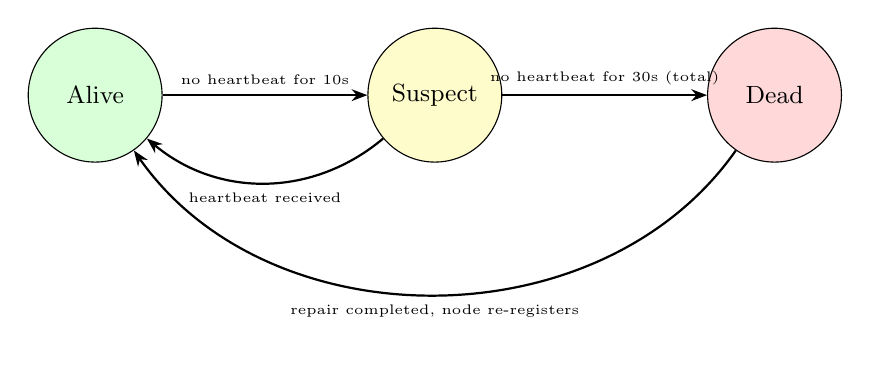
\begin{tikzpicture}[
    node distance=2.6cm,
    state/.style={draw, circle, minimum size=1.7cm, align=center, font=\small},
    arrow/.style={-{Stealth[length=2mm]}, thick}
]
    \node[state, fill=green!15] (alive) {Alive};
    \node[state, fill=yellow!20, right=of alive] (suspect) {Suspect};
    \node[state, fill=red!15, right=of suspect] (dead) {Dead};

    \draw[arrow] (alive) -- node[above, font=\tiny, align=center]{no heartbeat for 10s} (suspect);
    \draw[arrow] (suspect) -- node[above, font=\tiny, align=center]{no heartbeat for 30s (total)} (dead);
    \draw[arrow] (suspect) to[bend left=40] node[below, font=\tiny, align=center]{heartbeat received} (alive);
    \draw[arrow] (dead) to[bend left=55] node[below, font=\tiny, align=center]{repair completed, node re-registers} (alive);
\end{tikzpicture}
\caption{Node liveness state machine driving failure detection and repair triggering.}
\label{fig:failstates}
\end{figure}

Storage nodes heartbeat to the metadata cluster every 3 seconds. A node with no heartbeat for 10 seconds is marked \emph{Suspect}; after 30 seconds it is marked \emph{Dead}, which triggers the metadata cluster to scan for chunks that were replicated on the dead node and enqueue repair jobs for them. Rather than have the metadata cluster open new outbound connections to healthy storage nodes (which would complicate its purely request/response role), repair jobs are \emph{piggybacked on heartbeat responses} sent to the surviving source nodes that already hold a healthy copy of the affected chunk. The source node then re-replicates the chunk to a newly chosen target using the same peer-to-peer replication path used during normal uploads. If a previously dead node later restarts and re-registers, any stale replicas it still holds are evicted during a reconciliation pass, keeping the recorded replica set consistent with reality. Algorithm~\ref{alg:repair} summarizes this loop.

\begin{algorithm}[h]
\caption{Failure Detection and Repair (Metadata Cluster)}
\label{alg:repair}
\begin{algorithmic}[1]
\Loop
    \State receive Heartbeat from node $N$
    \State update last-seen timestamp for $N$
    \State $\textit{jobs} \gets$ pending repair jobs sourced from $N$ \Comment{piggybacked, not a separate RPC}
    \State respond to $N$ with $\textit{jobs}$
\EndLoop
\Statex
\Procedure{WatcherTick}{}
    \ForAll{registered node $N$}
        \If{now $-$ lastSeen($N$) $> 10$s \textbf{and} $N$ is Alive}
            \State mark $N$ as Suspect
        \ElsIf{now $-$ lastSeen($N$) $> 30$s \textbf{and} $N$ is Suspect}
            \State mark $N$ as Dead
            \ForAll{chunk $c$ replicated on $N$}
                \State choose surviving replica $s$ of $c$ as repair source
                \State choose new target node $t$ (most free space, not already holding $c$)
                \State enqueue repair job $(c, s, t)$
            \EndFor
        \EndIf
    \EndFor
\EndProcedure
\end{algorithmic}
\end{algorithm}

\section{Placement Strategy}

When placing a new chunk's primary and replicas, the metadata cluster selects nodes with the most free space, excludes nodes already holding a copy of the chunk, and avoids assigning two replicas of the same chunk to the same node. This is a simple greedy heuristic; Section~\ref{sec:limitations} discusses its main limitation (lack of rack/zone awareness).

\section{Consistency Model}

The system deliberately adopts a \textbf{write-once, read-many} consistency model: files cannot be updated or appended to after creation, and there is no distributed locking. This sidesteps the substantial complexity of concurrent-write ordering (e.g. GFS's lease-based primary election per chunk for mutation ordering) while still requiring genuine solutions to consensus, replication, and failure recovery for the write-once and read paths. Metadata operations are strongly consistent (linearizable through the Raft leader); a chunk is only exposed to clients as durable once it has been replicated to quorum and \texttt{CommitChunk} has been recorded in the metadata log.

% =====================================================
\chapter{Experimental Details}
% =====================================================

\section{Testing Methodology}

Distributed systems are usually validated at multiple layers of a testing pyramid: unit tests (pure logic, in-memory, fast), component tests (a single node against mocked dependencies), integration tests (multiple real nodes talking over real gRPC), and end-to-end or chaos tests (a realistic cluster with deliberate fault injection). This project follows that same pyramid, using in-process integration test harnesses similar to the pattern used by etcd, CockroachDB, and HashiCorp Consul/Nomad. These start real \texttt{MetadataNode} and \texttt{StorageNode} instances inside a single \texttt{go test} process on OS-assigned ports, which avoids the overhead and non-determinism of Docker-based test clusters while still exercising real gRPC and real Raft code paths.

\section{Test Scenarios Implemented}

Table~\ref{tab:tests} summarizes the integration test suites present in the repository, grouped by what they validate.

\begin{table}[h]
\centering
\footnotesize
\begin{tabular}{@{}p{2.2cm}p{6cm}p{6.3cm}@{}}
\toprule
\textbf{Test Suite} & \textbf{Representative Cases} & \textbf{What it Validates} \\
\midrule
Registration \& Heartbeat &
\texttt{\seqsplit{TestStorageNodesAutoRegistered}}, \texttt{\seqsplit{TestHeartbeatSucceeds}}, \texttt{\seqsplit{TestNodeDeregistration}}
&
Nodes correctly join the cluster and are tracked as live \\[4pt]

Upload / Download &
\texttt{\seqsplit{TestUploadAndDownloadSingleChunk}}, \texttt{\seqsplit{TestUploadWithReplication}}, \texttt{\seqsplit{TestFullUploadDownloadRoundTrip}}
&
Full \texttt{CreateFile}$\to{}$\allowbreak\texttt{PutChunk}$\to{}$\allowbreak\texttt{CommitChunk}$\to{}$\allowbreak\texttt{GetFile}$\to{}$\allowbreak\texttt{GetChunk} round trip \\[4pt]

Chunk-size Boundaries &
\texttt{\seqsplit{TestCreateFileRejectsZeroChunkSize}}, \texttt{\seqsplit{TestCreateFileRejectsOversizedChunkSize}}, \texttt{\seqsplit{TestMultiChunkDownloadOffsetCorrectness}}
&
Correct validation and byte-offset handling at chunk boundaries \\[4pt]

Checksum Integrity &
\texttt{\seqsplit{TestChunkVerifyAfterUpload}}, \texttt{\seqsplit{TestCommitFileStoresChecksum}}
&
SHA256 checksums correctly computed, stored, and verified \\[4pt]

Replication \& Repair &
\texttt{\seqsplit{TestUnderReplicationDetected}}, \texttt{\seqsplit{TestUnderReplicationTriggersRepair}}, \texttt{\seqsplit{TestRepairDoesNotLoop}}, \texttt{\seqsplit{TestRepairAfterNodeDeathConverges}}
&
Repair jobs are correctly triggered on under-replication and converge without looping \\[4pt]

Leader Failover &
\texttt{\seqsplit{TestFollowerRedirect\_ReturnsFailedPrecondition}}, \texttt{\seqsplit{TestLeaderCrash\_ClientRecovers}}, \texttt{\seqsplit{TestLeaderCrash\_ReadAfterFailover}}
&
Raft leader crash is transparently recovered from by the client \\[4pt]

End-to-End Client &
\texttt{\seqsplit{TestClientE2E\_SmallFileUploadDownload}}, \texttt{\seqsplit{TestClientE2E\_MultiChunkUploadDownload}}, \texttt{\seqsplit{TestClientE2E\_ChecksumIntegrity}}
&
Full client library behavior against a live cluster \\
\bottomrule
\end{tabular}
\caption{Integration test suites and the failure/behavior classes they cover (65 test cases total across the \texttt{integration/} package).}
\label{tab:tests}
\end{table}

\section{Representative Scenario: Node-Failure Repair}

The most illustrative test, \texttt{TestRepairAfterNodeDeathConverges}, exercises the full failure-and-recovery loop end to end:
\begin{enumerate}[nosep]
    \item A file is uploaded with a replication factor of 2 across two storage nodes.
    \item One storage node is stopped mid-test to simulate a crash.
    \item The test waits past the Suspect and Dead timeouts configured for the test cluster.
    \item A subsequent heartbeat from the surviving node is checked to confirm it carries a non-empty repair job for the chunk that was lost.
    \item The system is then checked for convergence, meaning repair does not keep re-triggering once the replication factor is restored (\texttt{TestRepairDoesNotLoop}).
\end{enumerate}

This validates the exact mechanism described in Algorithm~\ref{alg:repair}: detection via timeout, repair-job creation, piggybacking on heartbeats, and convergence.

\section{Running the Test Suite}

The test suite is isolated from normal unit tests using a Go build tag, and can be run with:
\begin{verbatim}
# Unit tests only
go test ./...

# Integration tests (real gRPC + real Raft, in-process cluster)
go test -tags integration -count=1 -timeout 120s ./integration/...
\end{verbatim}

Running the suite produces the following output (abbreviated to package-level summaries):

\begin{verbatim}
$ go test -tags integration -count=1 -timeout 120s ./integration/...
ok   github.com/satyam709/distributed-fs/integration/e2e           4.542s
ok   github.com/satyam709/distributed-fs/integration/failover      32.946s
ok   github.com/satyam709/distributed-fs/integration/meta_storage  111.671s
\end{verbatim}

All 65 integration tests (11 end-to-end client tests, 14 leader/follower failover tests, and 40 metadata--storage interaction tests) pass. Total wall-clock time is approximately 150 seconds on a single development machine (Ubuntu, 16~GB RAM, SSD storage). The \texttt{failover} and \texttt{meta\_storage} suites account for most of the elapsed time because they deliberately wait past heartbeat and suspect/dead timeouts to exercise the failure-detection and repair paths.

% =====================================================
\chapter{Conclusion and Future Work}
% =====================================================

\section{Conclusion}

This project implements a working, testable distributed file system that demonstrates the core mechanisms underlying production-grade distributed storage systems: Raft-based consensus for strongly consistent metadata, quorum-based peer-to-peer chunk replication, a heartbeat-driven failure detector with automatic self-healing, and a clean separation of concerns across three gRPC service boundaries. Rather than treating these as textbook abstractions, the project required making, and living with, the same category of engineering trade-offs that GFS, HDFS, and similar systems make: fixed vs. variable chunk sizing, where to place checksums, how aggressively to schedule repair work, and how to keep the metadata path from becoming a bottleneck. The extensive integration test suite, covering registration, full upload/download round trips, chunk-boundary edge cases, checksum verification, replication/repair convergence, and Raft leader failover, gives concrete evidence that these mechanisms actually behave correctly under simulated failure, and not just in the happy path.

The entire source code for this project is publicly available on GitHub at \url{https://github.com/Satyam709/distributed-fs} under the GNU General Public License v3.0 (GPL-3.0). The repository includes all application code, Protocol Buffer definitions, integration tests, and build instructions needed to reproduce the system and its test results.

\section{Limitations}
\label{sec:limitations}

In the interest of scope and honesty, the current system has the following known limitations:
\begin{itemize}[nosep]
    \item \textbf{Write-once semantics:} files cannot be updated or appended to after creation; there is no support for concurrent writers or distributed locking.
    \item \textbf{No rack/zone awareness:} the placement strategy selects nodes purely by free space, without regard to physical failure domains, so all replicas of a chunk could in principle share a single point of failure (e.g. a rack or power circuit) in a real deployment.
    \item \textbf{No transport security:} inter-node and client-node gRPC traffic is unauthenticated and unencrypted (no mTLS), which is acceptable for an academic prototype but not for production use.
    \item \textbf{Single metadata cluster:} there is no support for cross-datacenter metadata federation or geo-replication.
    \item \textbf{No storage quotas or access control.}
\end{itemize}

\section{Future Work}

Natural extensions include: rack-aware placement that spreads replicas across explicit failure domains; mutual TLS and basic authentication/authorization between all components; support for file appends via a lease-based mutation-ordering protocol similar to GFS's; erasure coding as a storage-efficient alternative to full replication for cold data; and a monitoring/visualization dashboard exposing cluster health, replication factor, and repair activity in real time.

% =====================================================
\begin{thebibliography}{9}

\bibitem{raft}
D. Ongaro and J. Ousterhout, ``In Search of an Understandable Consensus Algorithm (Extended Version),'' \textit{Proceedings of the 2014 USENIX Annual Technical Conference (USENIX ATC 14)}, 2014.

\bibitem{gfs}
S. Ghemawat, H. Gobioff, and S.-T. Leung, ``The Google File System,'' \textit{Proceedings of the 19th ACM Symposium on Operating Systems Principles (SOSP '03)}, 2003, pp. 29--43.

\bibitem{hdfs}
K. Shvachko, H. Kuang, S. Radia, and R. Chansler, ``The Hadoop Distributed File System,'' \textit{Proceedings of the 2010 IEEE 26th Symposium on Mass Storage Systems and Technologies (MSST)}, 2010.

\bibitem{hashicorpraft}
HashiCorp, \textit{raft: Golang implementation of the Raft consensus protocol}. [Online]. Available: \url{https://github.com/hashicorp/raft}

\bibitem{grpc}
Google, \textit{gRPC: A high-performance, open-source universal RPC framework}. [Online]. Available: \url{https://grpc.io}

\bibitem{bbolt}
etcd-io, \textit{bbolt: An embedded key/value database for Go}. [Online]. Available: \url{https://github.com/etcd-io/bbolt}

\bibitem{bittorrent}
B. Cohen, ``Incentives Build Robustness in BitTorrent,'' \textit{Workshop on Economics of Peer-to-Peer Systems}, 2003.

\end{thebibliography}

\end{document}